\chapter{Extra Results \& Control Plots}
	\label{ap:contol}

	This appendix contains additional plots from the data background comparison plots. Figure \ref{fig:afb_alt} shows the same A$_{FB}$ distribution as in the main text but with a different example signal overlaid. Figures \ref{fig:app_pt} and \ref{fig:app_eta} show the p$_{T}$ and $\eta$ distributions for the highest and second highest p$_{T}$ electrons with comparison between background and data. Figures \ref{fig:cosTS_1}, \ref{fig:cosTS_2}, \ref{fig:cosTS_3}, \ref{fig:cosTS_4} and \ref{fig:cosTS_5} show the comparison within the $\cos{\theta^{*}}$ variable for each of the search bins.


	\begin{figure}[ht]
		\centering
			\includegraphics[width=0.98\linewidth]{images/AFB_main_alt.eps}
		\caption{A$_{FB}$ comparison between data and MC with alternate signal overlay of CI. Ratio shows the difference between data and background prediction divided by total background systematic.}
		\label{fig:afb_alt}
	\end{figure}








	\begin{figure}[ht]
		\centering
			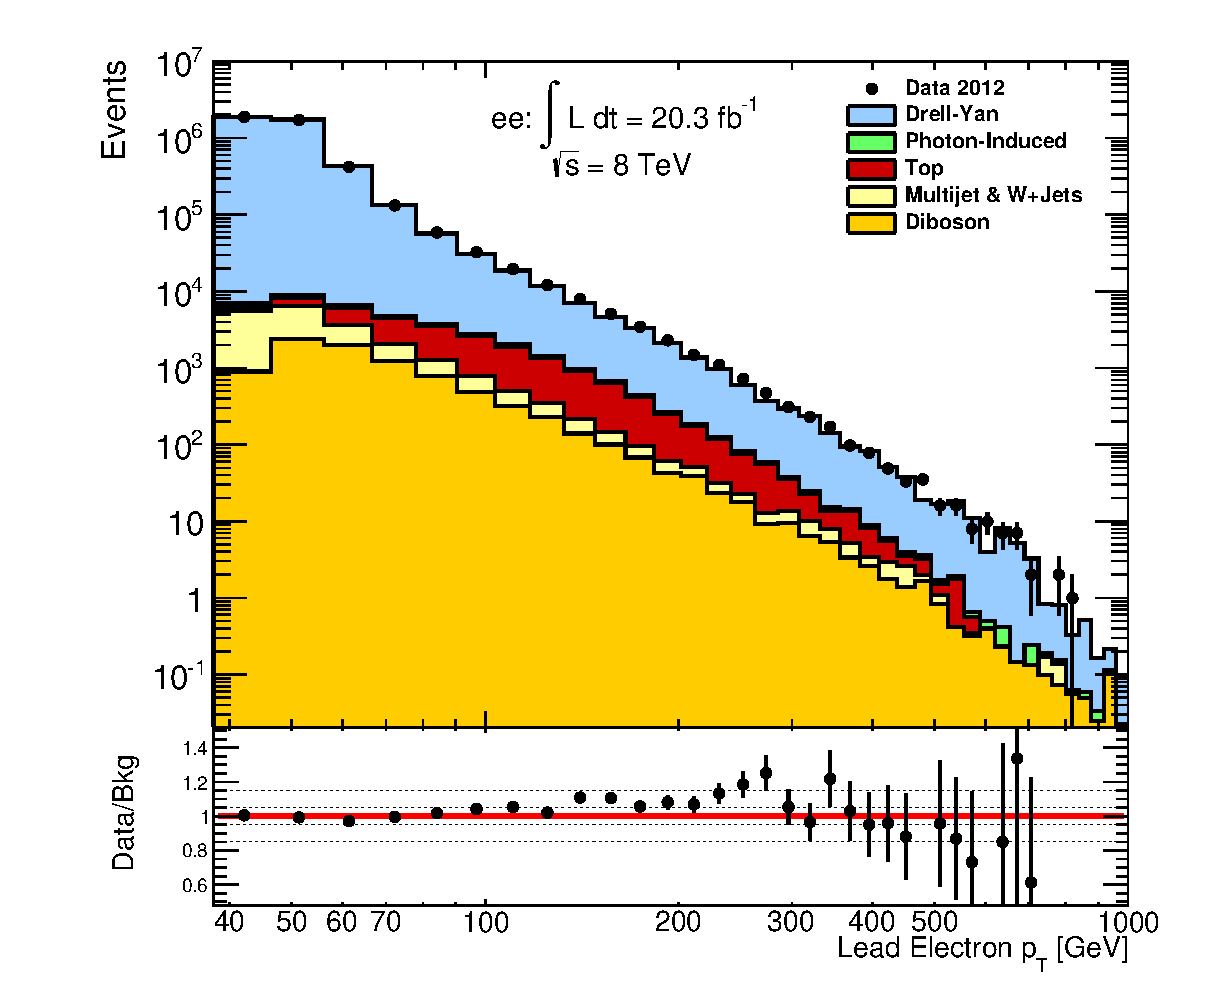
\includegraphics[width=0.49\linewidth]{images/pT_lead.eps}
			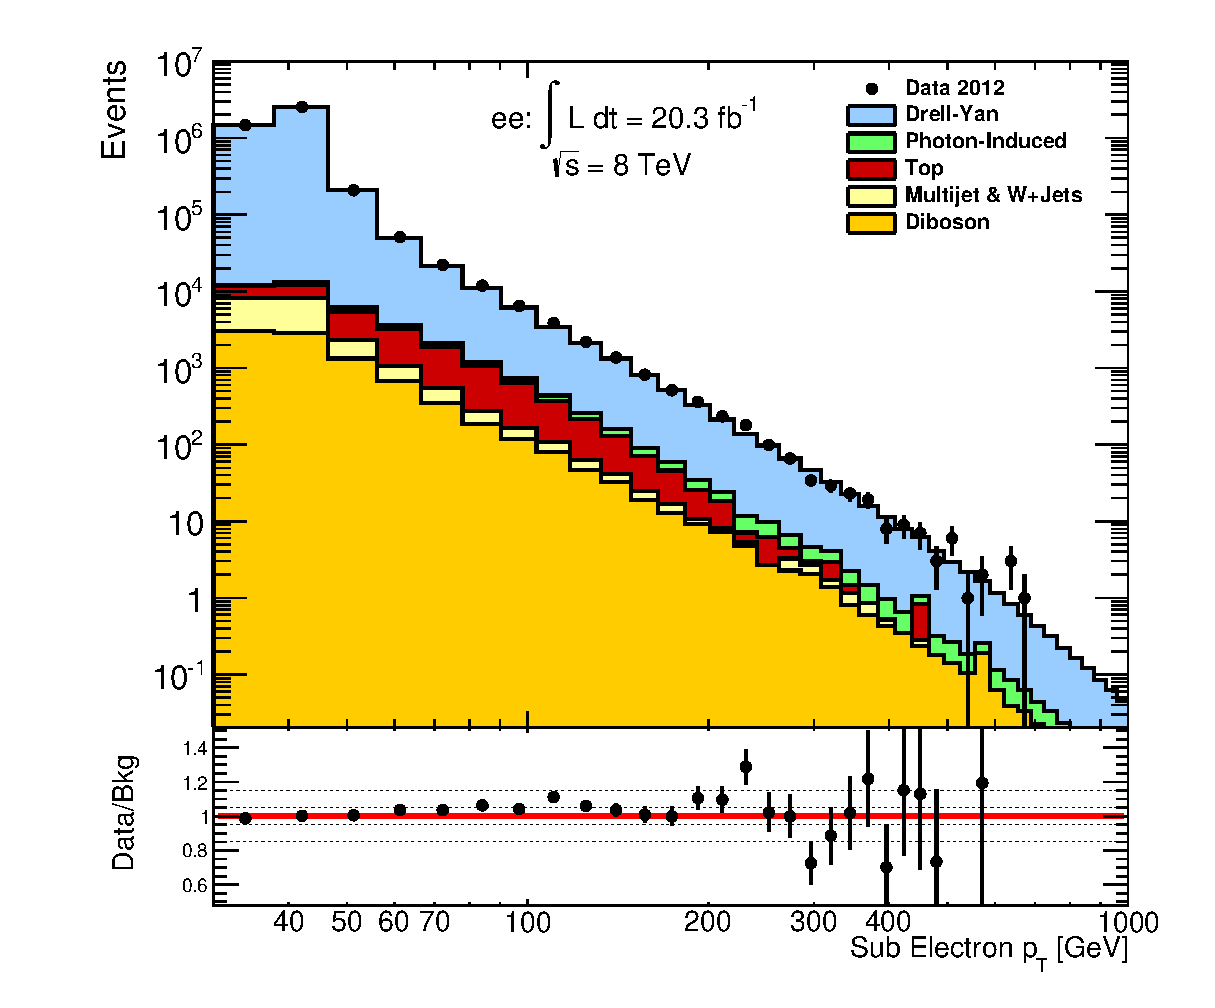
\includegraphics[width=0.49\linewidth]{images/pT_sub.eps}
		\caption{Distribution of p$_{T}$ of the selected highest (left) and second highest (right) p$_{T}$ electrons comparing data to background prediction.}
		\label{fig:app_pt}
	\end{figure}




	\begin{figure}[ht]
		\centering
			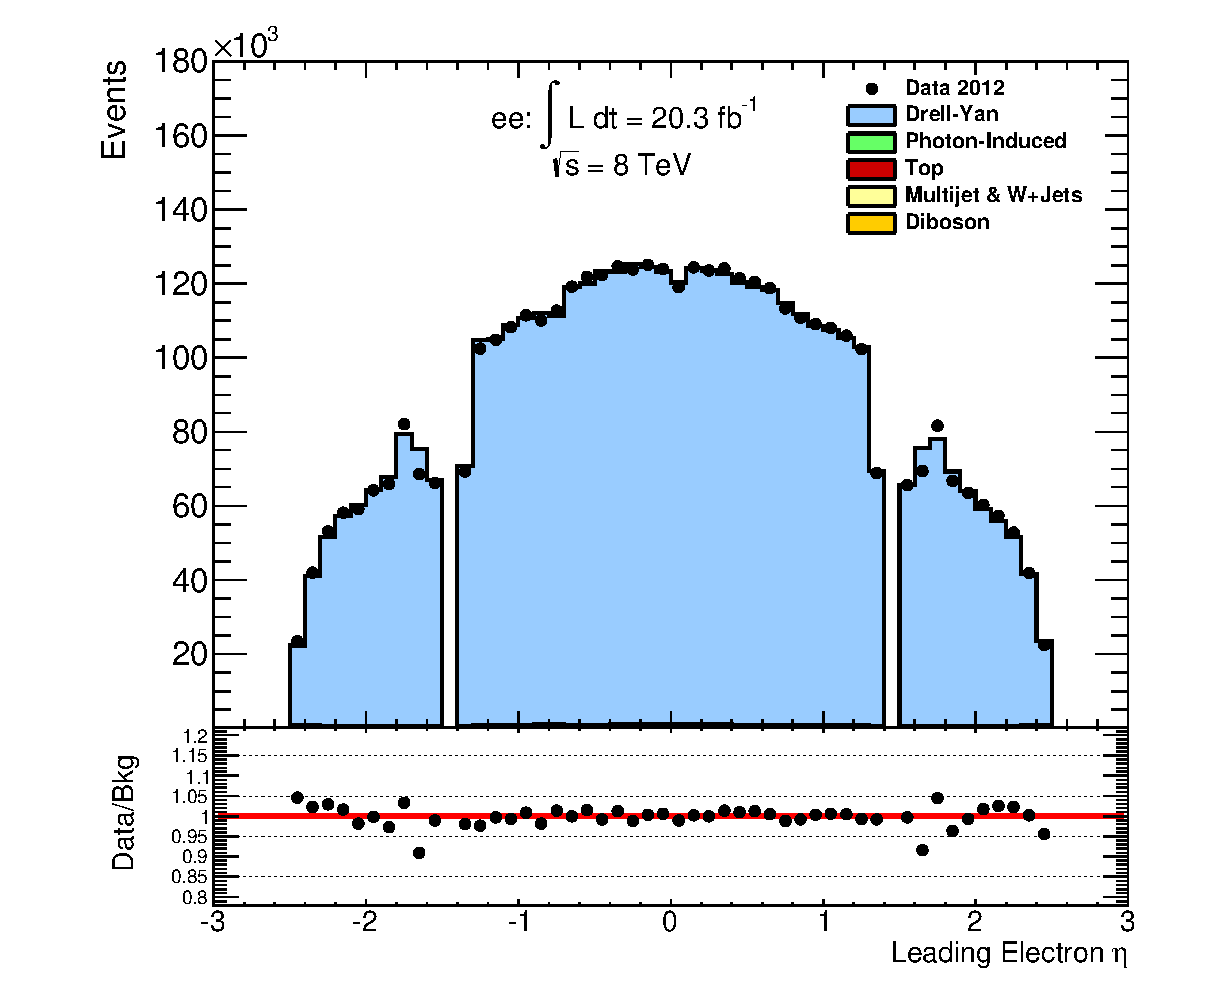
\includegraphics[width=0.49\linewidth]{images/eta_lead.eps}
			\includegraphics[width=0.49\linewidth]{images/eta_sub.eps}
		\caption{Distribution of $\eta$ of the selected highest (left) and second highest (right) p$_{T}$ electrons comparing data to background prediction.}
		\label{fig:app_eta}
	\end{figure}




	% \begin{figure}[ht]
	% 	\centering
	% 		\includegraphics[width=0.9\linewidth]{images/}
	% 	\caption{Distribution of $\phi$ of the selected highest and second highest p$_{T}$ electrons comparing data to background prediction.}
	% 	\label{fig:app_phi}
	% \end{figure}






	\begin{figure}[ht]
		\centering
			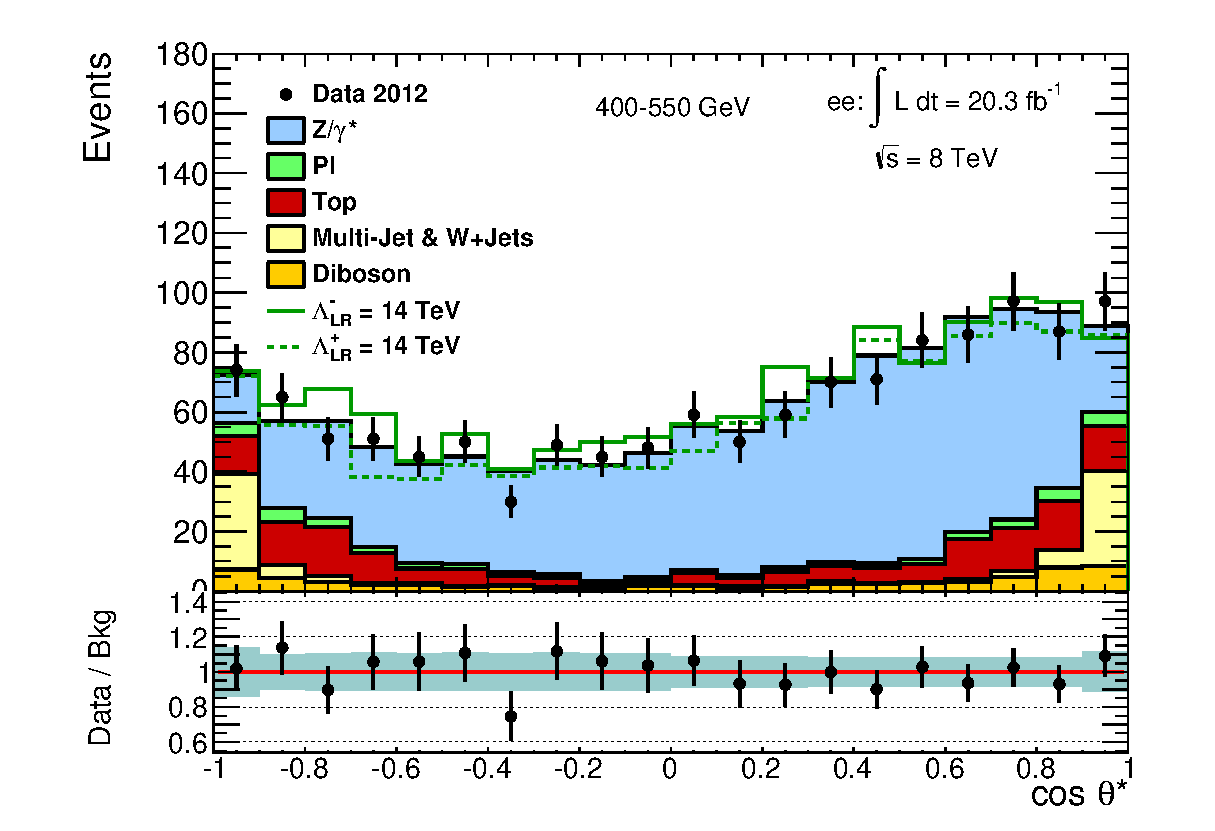
\includegraphics[width=0.9\linewidth]{images/CosThetaStar_bin_1.eps}
		\caption{Plot of $\cos{\theta^{*}}$ comparing background to data in the invariant mass search bin 400-550 GeV with signal overlay.}
		\label{fig:cosTS_1}
	\end{figure}

	\begin{figure}[ht]
		\centering
			\includegraphics[width=0.9\linewidth]{images/CosThetaStar_bin_2.eps}
		\caption{Plot of $\cos{\theta^{*}}$ comparing background to data in the invariant mass search bin 550-800 GeV with signal overlay.}
		\label{fig:cosTS_2}
	\end{figure}


	\begin{figure}[ht]
		\centering
			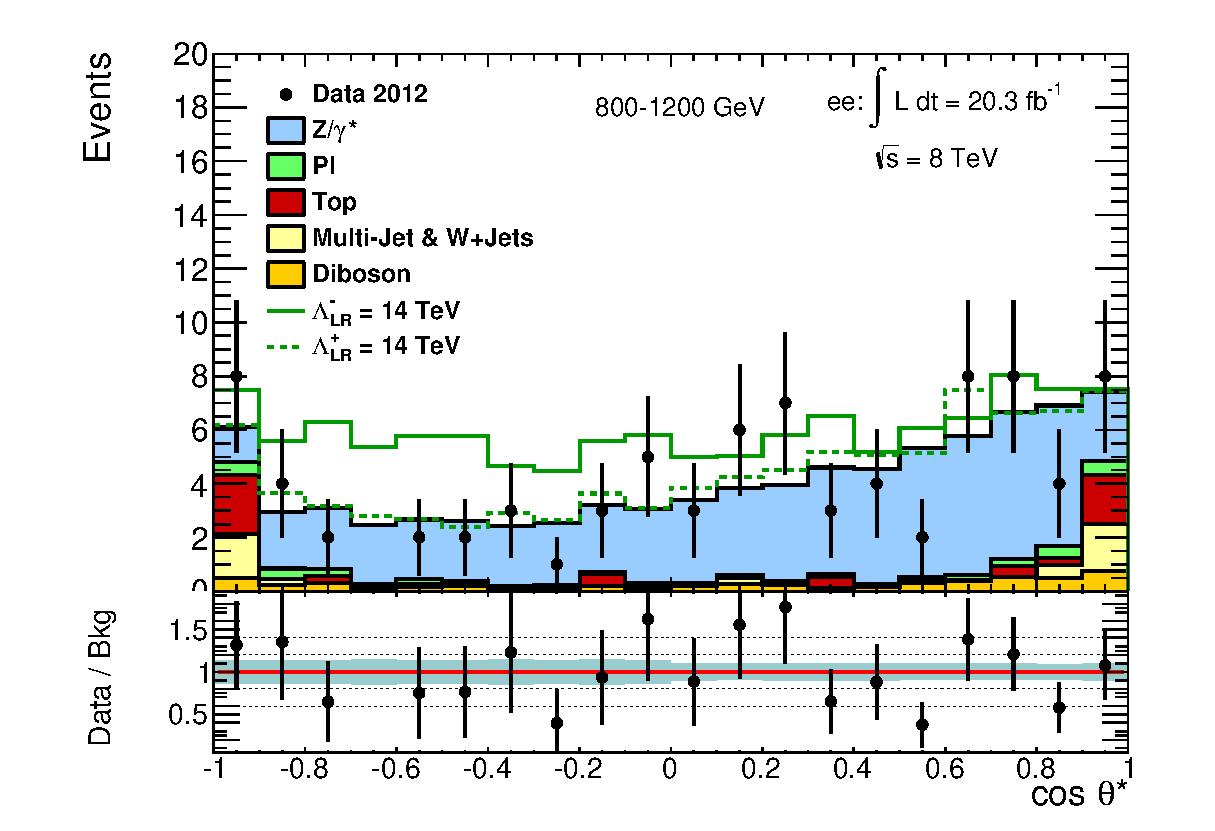
\includegraphics[width=0.9\linewidth]{images/CosThetaStar_bin_3.eps}
		\caption{Plot of $\cos{\theta^{*}}$ comparing background to data in the invariant mass search bin 800-1200 GeV with signal overlay.}
		\label{fig:cosTS_3}
	\end{figure}


	\begin{figure}[ht]
		\centering
			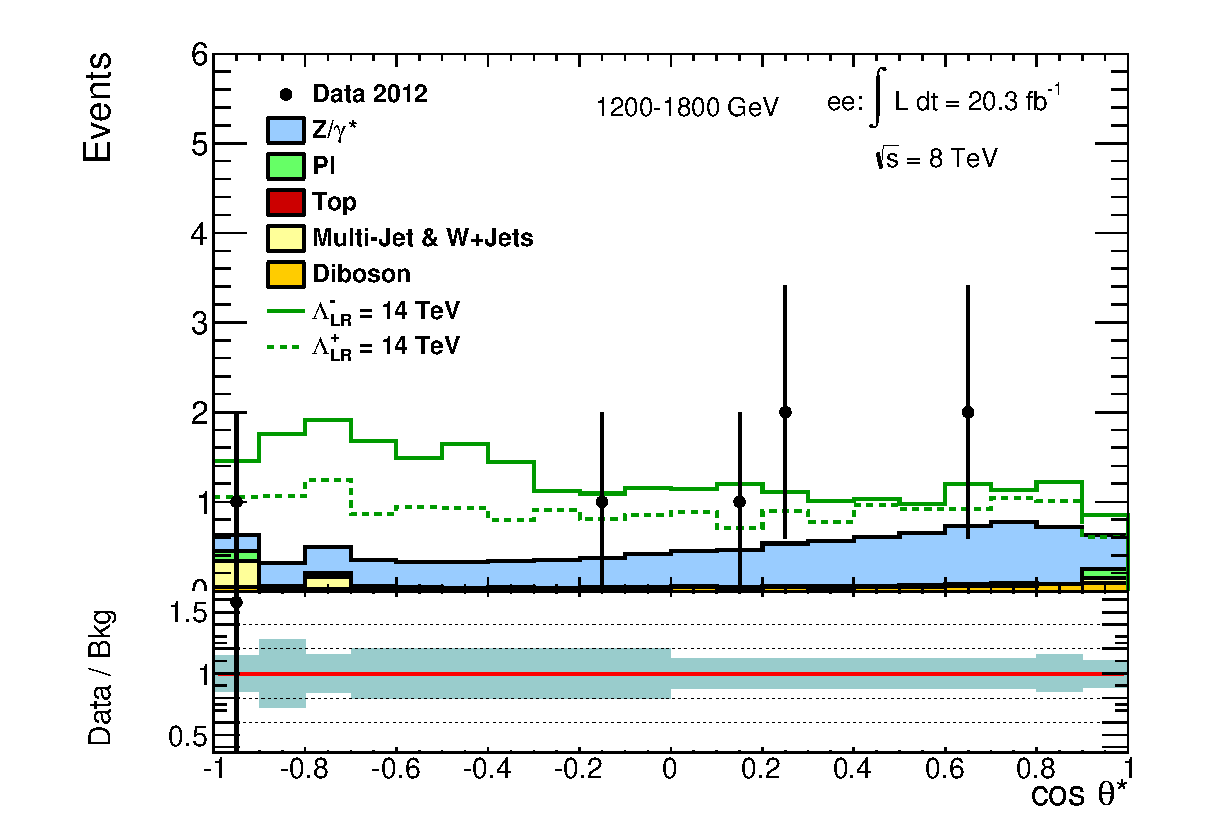
\includegraphics[width=0.9\linewidth]{images/CosThetaStar_bin_4.eps}
		\caption{Plot of $\cos{\theta^{*}}$ comparing background to data in the invariant mass search bin 1200-1800 GeV with signal overlay.}
		\label{fig:cosTS_4}
	\end{figure}


	\begin{figure}[ht]
		\centering
			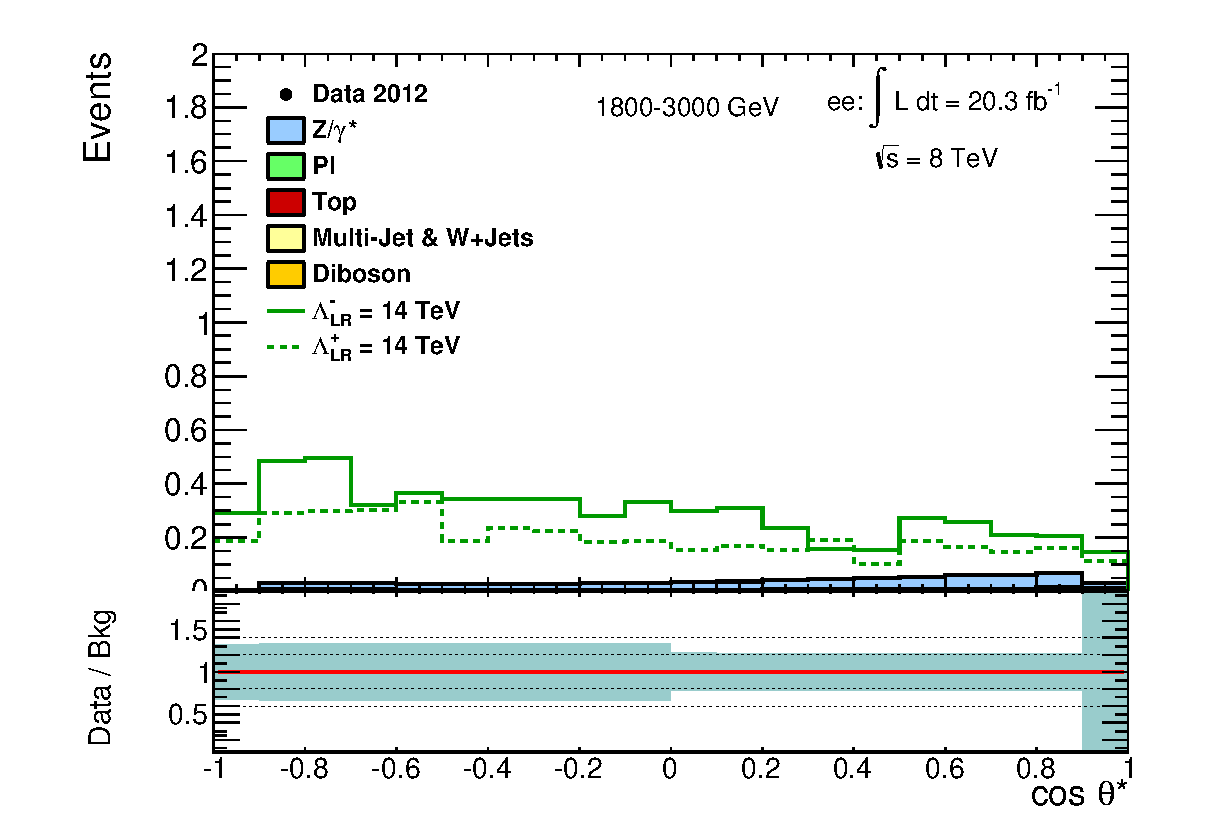
\includegraphics[width=0.49\linewidth]{images/CosThetaStar_bin_5.eps}
			\includegraphics[width=0.49\linewidth]{images/CosThetaStar_bin_6.eps}
		\caption{Plot of $\cos{\theta^{*}}$ comparing background to data in the invariant mass search bins 1800-3000 GeV and 3000-4500 GeV with signal overlay.}
		\label{fig:cosTS_5}
	\end{figure}






